\documentclass{article}

\usepackage{PRIMEarxiv}

\usepackage[
  pdfauthor={Khor Kean Teng},
  pdftitle={Alternative Assessment},
  pdfsubject={WQF7007 Natural Language Processing},
  pdfcreator={texlive},
  pdfproducer={LaTeX with hyperref},
]{hyperref}
\usepackage{url}
\usepackage{booktabs} % professional-quality tables
\usepackage[utf8]{inputenc} % allow utf-8 input
\usepackage[T1]{fontenc}    % use 8-bit T1 fonts
\usepackage{microtype}
\usepackage{fancyhdr}
\usepackage[style=apa, url=true, doi=true, eprint=false]{biblatex}
\addbibresource{references.bib} % Link to your .bib file
%\usepackage[margin=1in]{geometry} % Removed to avoid option clash
\usepackage{graphicx} % For including images
\usepackage{rotating}

\makeatletter
\renewbibmacro*{cite:author}{%
  \iffieldequals{namehash}{\cbx@lasthash}
% Multiple cites in one command
   {\setunit{\compcitedelim}%
    \printtext[bibhyperref]{%
      \usebibmacro{cite:plabelyear+extradate}}}%
% Single cite
   {\printtext[bibhyperref]{%
      \ifnameundef{labelname}
% No author/editor
       {\usebibmacro{cite:noname}%
         \savefield{namehash}{\cbx@lasthash}}
% Normal cite
       {\ifnameundef{shortauthor}
         {\printnames{labelname}}%
         {\cbx@apa@ifnamesaved
            {\printnames{shortauthor}}
            {\printnames[labelname]{author}%
             \addspace\printnames[sabrackets]{shortauthor}}}%
          \savefield{namehash}{\cbx@lasthash}}}}%
   \setunit{\multicitedelim}}

\renewbibmacro*{cite}{%
  \iffieldequals{namehash}{\cbx@lasthash}
% Multiple cites in one command
   {\setunit{\compcitedelim}%
    \printtext[bibhyperref]{%
      \usebibmacro{cite:plabelyear+extradate}}}%
% Single cite
   {\printtext[bibhyperref]{%
      \ifnameundef{labelname}
% No author/editor
       {\usebibmacro{cite:noname}%
         \setunit{\printdelim{nameyeardelim}}%
         \usebibmacro{cite:plabelyear+extradate}%
         \savefield{namehash}{\cbx@lasthash}}
% Normal cite
       {\ifnameundef{shortauthor}
         {\printnames{labelname}}%
         {\cbx@apa@ifnamesaved
           {\printnames{shortauthor}}
           {\printnames[labelname]{author}%
            \addspace\printnames[sabrackets]{shortauthor}}}%
         \setunit{\printdelim{nameyeardelim}}%
        \usebibmacro{cite:plabelyear+extradate}%
        \savefield{namehash}{\cbx@lasthash}}}}%
   \setunit{\multicitedelim}}

\renewbibmacro*{textcite}{%
  \iffieldequals{namehash}{\cbx@lasthash}
% Compact cite - more than one thing for same author
    {\setunit{\compcitedelim}%
     \printtext[bibhyperref]{%
       \usebibmacro{cite:plabelyear+extradate}}}
% New cite
    {\ifbool{cbx:parens}
       {\bibcloseparen\global\boolfalse{cbx:parens}}
       {}%
     \setunit{\textcitedelim}%
     \ifnameundef{labelname}
     % No author/editor
       {\iffieldundef{shorthand}%
    % Cite using title
         {\printtext[bibhyperref]{\usebibmacro{cite:noname}}%
          \setunit{\global\booltrue{cbx:parens}%
                   \printdelim{nonameyeardelim}%
                   \bibopenparen}%
          \printtext[bibhyperref]{%
            \usebibmacro{cite:plabelyear+extradate}}}
    % Cite using shorthand
         {\printtext[bibhyperref]{%
            \usebibmacro{cite:shorthand}}}}
  % Normal cite with author/editor
  % Normal full cite
       {\printtext[bibhyperref]{%
          \ifnameundef{shortauthor}%
    % Normal full cite
           {\printnames{labelname}}
    % Cite using short author
           {\cbx@apa@ifnamesaved
             {\printnames{shortauthor}}
             {\printnames[labelname]{author}}}}%
  % Year
        \setunit{\global\booltrue{cbx:parens}%
                 \printdelim{nameyeardelim}%
                 \bibopenparen}%
  % Put the shortauthor inside the year brackets if necessary
        \printtext[bibhyperref]{%
          \ifnameundef{shortauthor}
           {}
           {\cbx@apa@ifnamesaved
             {}
             {\printnames{shortauthor}%
              \setunit{\printdelim{innernameyeardelim}}}}%
  % Print prenote (belongs to first cite)
        \ifnumequal{\value{citecount}}{1}
           {\usebibmacro{prenote}}
           {}%
  % Actual year printing
        \usebibmacro{cite:plabelyear+extradate}%
  % Save name hash for checks later
        \savefield{namehash}{\cbx@lasthash}}%
    \stepcounter{textcitecount}}}}

\renewbibmacro*{cite:plabelyear+extradate}{%
  \iffieldundef{labelyear}{}
    {\clearfield{labelmonth}% don't want months in citations
     \clearfield{labelday}% don't want days in citations
     \clearfield{labelendmonth}% don't want months in citations
     \clearfield{labelendday}% don't want days in citations
     \clearfield{labelyeardivision}% don't want yeardivisions in citations
     \clearfield{labelendyeardivision}% don't want yeardivisions in citations
     \iffieldsequal{labelyear}{labelendyear}% Don't want no-op year ranges
       {\clearfield{labelendyear}}
       {}%
     \iffieldundef{origyear}
       {}
       {\printorigdate%
        \setunit*{\addslash}}%
     \iffieldundef{related}
       {}
       {\iffieldequalstr{relatedtype}{reprintfrom}
         {\entrydata*{\thefield{related}}{\printlabeldateextra}%
          \setunit*{\addslash}}
         {}}%
     \printlabeldateextra}}

\renewbibmacro*{citeyear}{%
  \iffieldundef{labelyear}
    {\usebibmacro{cite:init}}
    {\iffieldequals{namehash}{\cbx@lasthash}
       {\setunit{\compcitedelim}%
        \printtext[bibhyperref]{\usebibmacro{cite:plabelyear+extradate}}}
       {\printtext[bibhyperref]{\usebibmacro{cite:plabelyear+extradate}}%
        \savefield{namehash}{\cbx@lasthash}}}%
  \setunit{\multicitedelim}}
\makeatother

%Header
\pagestyle{fancy}
\thispagestyle{empty}
\rhead{ \textit{ }} 

% Update your Headers here
\fancyhead[LO]{Alternative Assessment}

%% Title
\title{Alternative Assessment}

\author{
  Khor Kean Teng \\
  WQF 7007 Natural Language Processing \\
  Faculty of Computer Science \& Information Technology, University Malaya \\
  \texttt{\{u2004763\}@siswa.um.edu.my} \\
}

\begin{document}

\maketitle

\section*{Question 1}

\textit{Explain TWO (2) shortcomings of Bag-of-Words (BoW) and TF-IDF features in sentiment analysis, supporting your explanation with relevant examples. In addition to Word Embeddings and Transformer-based methods, suggest at least TWO (2) other alternative approaches that can help overcome these limitations. Use linguistic examples to clarify your suggestions.}

\begin{center}
  $\ast$~$\ast$~$\ast$
\end{center}

BoW represents text as a vector of word frequencies, ignoring word order, while TF-IDF weights these frequencies by the rarity of words across documents. Both are widely used in sentiment analysis, which involves classifying text as positive, negative, or neutral. However, their simplicity can lead to significant shortcomings, particularly in capturing the nuances of human language.

One of the shortcomings of BoW and TF-IDF is loss of word order and context. For instance, BoW and TF-IDF treat text as an unordered collection, disregarding grammar and syntax. This is particularly problematic for sentiment analysis, where context is crucial. For instance, consider the sentences \textbf{"I like the person called Maya"} and \textbf{"I do not like the person called Maya."} In BoW, both might have similar word counts for \textbf{"like"} \textbf{"person"} etc., but the presence of \textbf{"not"} in the second sentence reverses the sentiment. In fact BoW and TF-IDF can misclassify negations without considering word order \parencite{mohey_enhancement_2016}. Another example is sarcasm or mixed sentiments, like "Oh great, another that's so bad." BoW might count "great" as positive, missing the ironic tone, which can lead to incorrect sentiment classification \parencite{brownlee_how_2020}.

Furthermore, BoW and TF-IDF struggles to capture semantic meaning. This is because they treat each word independently, without understanding semantic relationships such as synonyms, antonyms, or sentiment intensity. For example, "good" and "excellent" both convey positive sentiment, but "excellent" implies a stronger positive intensity. BoW would represent them as separate features, potentially leading to models that fail to generalize across similar meanings. This was identified as a major weakness in an academic paper, which noted that BoW ignores semantics, affecting sentiment analysis accuracy \parencite{mohey_enhancement_2016}. Another example is polysemy, where a word like "bank" can mean a financial institution (potentially neutral or negative in sentiment) or the side of a river (neutral). Without semantic understanding, BoW might misinterpret the context. Additionally, the high dimensionality of BoW vectors, often sparse due to many zero values, can make it harder for models to learn effectively \parencite{brownlee_how_2020}.

Some alternatives to overcome the identified shortcomings are n-grams and sentiment lexicons. Considering N-grams that involve using sequences of words, such as bigrams (two words) or trigrams (three words), they can capture local context and word order. This approach can address the loss of context by including phrases that carry sentiment, such as negations or intensifiers. For example, in the sentence \textbf{"Maya is not beautiful"}, the bigram \textbf{"not beautiful"} can be a feature that indicates negative sentiment, whereas in \textbf{"Maya is a beautiful person"}, the bigram \textbf{"beautiful person"} might indicate positive sentiment. Moreover, N-grams also help with sentiment intensity, as phrases like "very good" (bigram: "very good") can indicate stronger positivity compared to just "good." This approach is particularly useful for handling idiomatic expressions and negations, addressing both shortcomings identified earlier.

Alternatively, think about sentiment lexicons which are dictionaries that assign sentiment scores to words, often with positive, negative, or neutral labels, and sometimes including intensity (e.g., -1 to +1). They can incorporate semantic meaning by providing predefined sentiment for words, addressing the second shortcoming. For example, words like "happy," "joy," and "excellent" might have high positive scores, while "sad," "bad," and "terrible" have negative scores. In a sentence like "The service was excellent," "excellent" would contribute a strong positive score, improving sentiment classification. That is not all, some lexicons also handle negations and intensifiers through rules, such as reversing the score if "not" precedes a word. For instance, in "The service was not excellent," the lexicon might adjust the score of "excellent" to negative, addressing the context issue to some extent. 

To recap, consider the sentence \textbf{"I thought Maya was beautiful, but it was ugly"}. BoW might count \textbf{"beautiful"} and \textbf{"ugly"} potentially averaging to neutral, missing the overall negative sentiment due to the contrast. Using n-grams, bigrams like \textbf{"was beautiful"} and \textbf{"was ugly"} could be features, and with appropriate weighting, the model might capture the negative conclusion. Similarly, a sentiment lexicon would score "beautiful" positively and "not" negatively, and rules could prioritize the latter for final sentiment, addressing both shortcomings. In addition, "The acting was great, but the plot was terrible." N-grams could include "acting great" (positive) and "plot terrible" (negative), while a lexicon would score "great" highly positive and "terrible" highly negative, allowing for aspect-based sentiment analysis.

In a nutshell, BoW and TF-IDF's limitations in sentiment analysis stem from their inability to handle word order and semantic relationships, as evidenced by examples like negations and sentiment intensity. Alternatives like n-grams and sentiment lexicons offer practical solutions, improving context and semantic understanding, respectively. These approaches, supported by recent research, provide robust methods for enhancing sentiment analysis accuracy.

\section*{Question 2}

\textit{Language modelling is a foundational task in Natural Language Processing (NLP), enabling applications such as machine translation, speech recognition, and text generation. While statistical approaches such as n-gram models dominated early research, the field has shifted significantly toward neural language models, particularly those based on the Transformer architecture.}

\subsection*{Part A}

\textit{Explain how n-gram models calculate the probability of a sequence of words. Compare this to how neural models estimate these probabilities. Facilitate your answer with examples.}

\begin{center}
  $\ast$~$\ast$~$\ast$
\end{center}

N-gram models are statistical language models that estimate the probability of a word sequence by relying on the Markov assumption \parencite{young_week_2024}. This assumption posits that the probability of a word depends only on a fixed number of preceding words ($n-1$ words).

Chain rule is applied to calculate the probability of a sequence of words, $P(w_1,w_2,\ldots,w_n)$:

$$P(w_1, w_2, \ldots, w_n) = P(w_1) \times P(w_2|w_1) \times P(w_3|w_1, w_2) \times \ldots \times P(w_m|w_1, \ldots, w_{n-1})$$

This formula states that the probability of a sequence is the product of the conditional probabilities of each word given its preceding words. However, calculating the exact conditional probabilities in the chain rule is difficult due to data sparsity - many sequences will not have occurred in the training data. N-gram models simplify this by approximating the history:

$$ P(w_i \mid w_1,\ldots,w_{i-1}) \approx P(w_i \mid w_{i-n+1},\ldots,w_{i-1}) $$

This means the probability of a word $w_i$ is approximated by its probability given the previous n-1 words. Of course, the probabilities themselves are typically estimated using Maximum Likelihood Estimation (MLE) from a large text corpus. For an n-gram, the probability is calculated as the count of the specific n-gram divided by the count of its prefix (the n-1 preceding words) \parencite{keselji_speech_2025}. For a bigram model, the probability of word $w_i$ given word $w_{i-1}$ is:

$$P(w_i | w_{i-1})=\frac{Count(w_{i-1},w_i )}{(Count(w_{i-1}) )}$$

Let's calculate the probability of the sentence "I love NLP" using a bigram model. Assume we have the following counts from a corpus:
\begin{itemize}
    \item Count(I) = 1000
    \item Count(I love) = 20
    \item Count(love) = 500
    \item Count(love NLP) = 50
    \item Count($\langle$s$\rangle$ I) = 300 (where $\langle$s$\rangle$ is a start-of-sentence token)
    \item Count(NLP $\langle$/s$\rangle$) = 20 (where $\langle$/s$\rangle$ is an end-of-sentence token)
    \item Count(NLP) = 100
\end{itemize}

Calculation:

\begin{itemize}
    \item $P(I love NLP) \approx P(I|<s>) * P(love|I) * P(NLP|love) * P(</s>|NLP)$
	\item $P(I|<s>) = Count(<s> I) / Count(<s>)$
	\item $P(love|I) = \frac{Count(I love)}{Count(I)} = 200 / 1000 = 0.2$
	\item $P(NLP|love) = \frac{Count(love NLP)}{Count(love)} = 50 / 500 = 0.1$
	\item $P(</s>|NLP) = \frac{Count(NLP </s>)}{Count(NLP)}$
\end{itemize}


However, the n-gram models suffered from sparsity and limited context issues where many n-grams will not appear in the training data, leading to zero probabilities. Smoothing techniques such as Laplace or Add-k smoothing, Good-Turing, Kneser-Ney are used to address this. Furthermore, N-grams only consider a fixed, short context ($n-1$ words), failing to capture long-range dependencies in language. Thus, advancement in neural language models (NLMs) overcome some limitations of n-gram models by learning distributed representations of words (word embeddings) and using neural networks to estimate word sequence probabilities.

Instead of relying on raw word counts, NLMs map words to dense vector representations (embeddings). These embeddings capture semantic and syntactic similarities between words, allowing the model to generalize better to unseen word combinations \parencite{bengio_neural_2003}. In recent decades, various neural network architectures are used, starting from feedforward neural network that takes a fixed-size window of previous words as input to predict the next word; Recurrent Neural Networks (RNNs) and Long Short-Term Memory (LSTMs) where RNNs are designed to process sequential data. They maintain a hidden state that theoretically captures information from all previous words in the sequence, allowing them to model longer-range dependencies than n-grams. On the other hand, LSTMs are a type of RNN specifically designed to better handle long-range dependencies by using gating mechanisms. Nowadays, modern state-of-the-art NLMs are predominantly based on the Transformer architecture. Transformers use a mechanism called "self-attention," which allows the model to weigh the importance of different words in the context (even distant ones) when predicting the next word.

NLMs typically predict the probability of the next word given the preceding context. The network processes the input sequence (or its embedding representation) and outputs a probability distribution over the entire vocabulary for the next word. This is often achieved using a SoftMax activation function in the output layer:

$$P(w_i|w_1,\ldots,w_{i-1} )=softmax(f(context(w_i,\ldots,w_{i-1} )))$$

\textit{*Note: $f$ is the neural network}

NLMs are trained on large text corpora to maximize the likelihood of the training data. This is typically done using variants of stochastic gradient descent and backpropagation, minimizing a loss function like cross-entropy. Let's do a thought experiment on how neural model works where we use the sentence \textbf{"I am falling in love with \_\_"}:

An NLM would first convert "I", "am", "falling", "in", "love", “with”, into their respective word embeddings. Then, these embeddings would be processed by the neural network be it an LSTM or a transformer. The network's internal state or attention mechanism would capture the contextual information. Finally, the output layer would produce a probability distribution over all words in the vocabulary. Words like \textbf{"Maya,"} \textbf{"Paris"}, or \textbf{"Latte"} would ideally receive higher probabilities than semantically, or syntactically implausible words like "bullshit" or "laziness".

\subsection*{Part B}

\textit{Identify and explain TWO (2) key limitations of statistical language models. Demonstrate how modern neural approaches address these limitations by providing relevant examples.}

\begin{center}
  $\ast$~$\ast$~$\ast$
\end{center}

Statistical language models while foundational to natural language processing, possess inherent limitations that have paved the way for more advanced neural network-based approaches. Two key limitations of are data sparsity and their restricted ability to capture long-range dependencies and complex contextual information. Modern neural approaches, such as Recurrent Neural Networks (RNNs) and Transformer models, have made significant strides in addressing these shortcomings.

Considering data sparsity, as noted in n-gram models when estimating the probability of a word occurring given its preceding n-1 words. A major challenge arises when a specific n-gram (a sequence of n words) has never or rarely appeared in the training corpus. This leads to zero or unreliable probability estimates for those unseen or rare sequences, a problem known as data sparsity. As the value of 'n' (the context window) increases to capture more context, the number of possible n-grams grows exponentially, making data sparsity an even more pronounced issue. This means the model struggles to generalize to new or less frequent word combinations, negatively impacting its predictive accuracy \parencite{dasgupta_hitgram_2024}.

To overcome this issue, Modern neural architectures, particularly RNNs (and their variants like LSTMs) and Transformer models, are designed to better capture sequential information and long-range dependencies. For instance, RNNs possess a "memory" in the form of a hidden state that allows them to retain information from previous inputs in a sequence. As an RNN processes a sentence word by word, its hidden state is updated, theoretically allowing it to capture information from earlier words to influence predictions for later words. LSTMs (Long Short-Term Memory networks), a special type of RNN, were specifically designed to combat the vanishing gradient problem, enabling them to learn and remember information over longer sequences. In the sentence, \textbf{"Maya, which I confessed to earlier, is now blushing"}, an RNN/LSTM can theoretically maintain information about "Maya" across the intervening clause "which I confessed to earlier" to correctly predict that "is" (singular verb) agrees with "Maya".

Admittedly, modern state-of-the-art language models are based on the transformer architecture. Transformers have revolutionized the handling of long-range dependencies through a mechanism called self-attention. Unlike RNNs that process words sequentially, transformers can process all words in a sequence simultaneously. The self-attention mechanism allows the model to weigh the importance of all other words in the input sequence when encoding a particular word. This means that for any given word, the model can directly "attend" to and draw context from any other word in the sequence, regardless of its distance. In a long paragraph discussing a specific concept introduced at the beginning, a Transformer model can use its self-attention mechanism to directly link later mentions of pronouns or related terms back to the original concept, even if they are many sentences apart. This allows for a more holistic understanding of the text and more contextually relevant predictions or generations.

Above all, while statistical language models laid crucial groundwork, modern neural approaches like RNNs and especially Transformers have significantly advanced the field by effectively mitigating issues of data sparsity through learned representations (embeddings) and by capturing more extensive contextual information and long-range dependencies through architectural innovations like recurrent states and self-attention mechanisms.

\subsection*{Part C}

\textit{Discuss why the Transformer architecture has been crucial for applying language modelling to very large datasets and in effectively capturing long range dependencies. Support your discussion by citing specific sections or experiments from at least TWO (2) recent peer-reviewed papers.}

\begin{center}
  $\ast$~$\ast$~$\ast$
\end{center}

Resources sourced from lectures videos published by one of the Professor in National Taiwan University, Hung-yi Lee with title: \textbf{[Generative AI] Large Models + Large Dataset = Magnificent Results?}

\begin{itemize}
    \item \url{https://www.youtube.com/watch?v=SaZTJJNOCOY}
    \item \url{https://www.youtube.com/watch?v=qycxA-xX_OY}
    \item \url{https://www.youtube.com/watch?v=V-3ksGCjehU}
\end{itemize}

Transformer architecture has emerged as a cornerstone in the evolution of language modeling, particularly when dealing with extensive datasets. Its prominence is attributed to inherent efficiencies in parallel processing and a robust capacity for capturing long-range dependencies within textual data. These characteristics have facilitated significant advancements in the scale and performance of language models.

\begin{figure}[htpb]
    \centering
    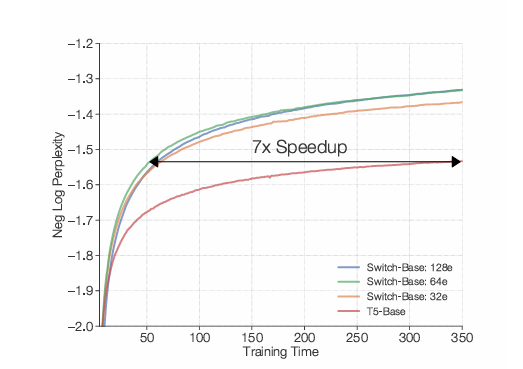
\includegraphics[width=0.6\textwidth]{../images/image-3.png} % Replace with your image path
    \caption{Speed advantage of Switch Transformer. All models trained on 32 TPUv3 cores with equal FLOPs per example. For a xed amount of computation and training time, Switch Transformers signi cantly outperform the dense Transformer baseline. Our 64 expert Switch-Base model achieves the same quality in one-seventh the time of the T5-Base and continues to improve}
    \label{fig:switch}
\end{figure}

A critical advantage of the Transformer architecture lies in its remarkable scalability and proficiency in managing large datasets. The architecture's self-attention mechanism is central to this capability, permitting the simultaneous processing of all tokens in an input sequence. This parallelism contrasts sharply with recurrent neural networks (RNNs), which process token sequentially, and is indispensable for the efficient training of contemporary language models on massive data corpora. Research by \parencite{kaplan_scaling_2020} established that model performance demonstrates a power-law relationship with model size, dataset size, and computational resources, and the Transformer architecture is pivotal in realizing such scaling. Building on this, \parencite{fedus_switch_2022} introduced sparsity through Switch Transformers, enabling the efficient training of models with over a trillion parameters. Their work highlighted that the Switch Transformer architecture could achieve up to a sevenfold increase in pre-training speed using equivalent computational resources by effectively leveraging hardware designed for dense matrix multiplications, thereby maximizing parameter count in a computationally efficient manner as shown in Fig \ref{fig:switch}. Further underscoring the importance of data and model scaling, \parencite{hoffmann_training_2022} determined that optimal training necessitates a proportional scaling of both model size and the number of training tokens, reinforcing the need for architectures like Transformers that can effectively process vast quantities of data. The practical manifestation of this scalability is exemplified by models such as Gopher, a 280 billion parameter model discussed by \parencite{rae_scaling_2022}, which showcases the Transformer's capacity to handle extremely large model dimensions as shown in Fig \ref{fig:gopher}.

\begin{figure}[htpb]
    \centering
    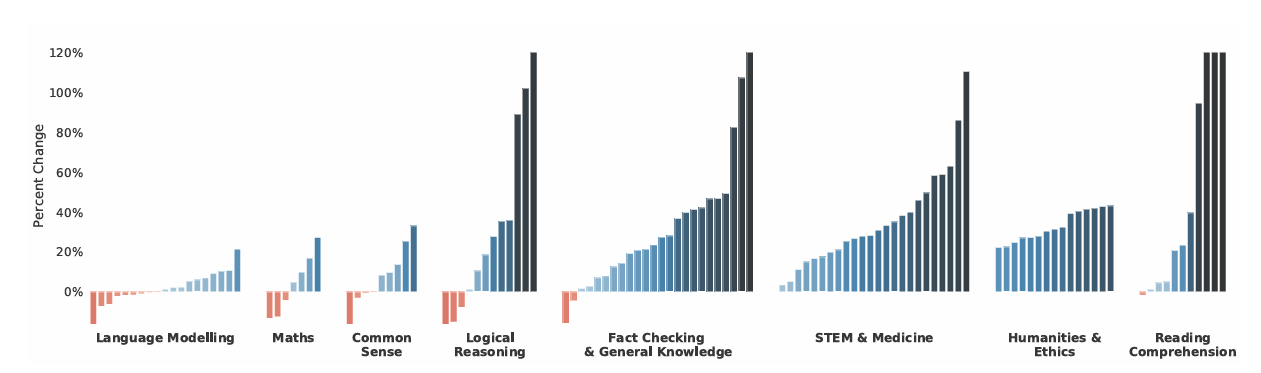
\includegraphics[width=0.6\textwidth]{../images/image-4.png} % Replace with your image path
    \caption{An overview of the percentage change in performance metric (higher is better) of Gopher versus state-of-the-art language model performance across 124 tasks. Each bar represents a task, here we clip the maximum relative improvement to 120\%. In total Gopher shows an improvement across 100 / 124. The best-published results include (175B) GPT-3, (178B) Jurassic-1, and (530B) Megatron-Turing NLG.}
    \label{fig:gopher}
\end{figure}

Beyond scalability, the Transformer's proficiency in capturing long-range dependencies—relationships between distant tokens in a sequence—is fundamental to its success. This ability is crucial for comprehending context and generating coherent, meaningful text. The self-attention mechanism allows each token to directly attend to all other tokens in the sequence, irrespective of their proximity. This direct pathway for information flow overcomes a significant limitation of RNNs, where information must traverse numerous intermediate steps, risking issues like vanishing gradients. While the foundational concept was introduced by \parencite{vaswani_attention_2023}, the empirical success of large-scale models such as Gopher and those analyzed by \parencite{kaplan_scaling_2020} across diverse tasks implicitly validates the Transformer's strength in this domain. These models consistently achieve high performance on tasks demanding deep contextual understanding, which inherently relies on the effective capture of long-range dependencies.

\begin{figure}[htpb]
    \centering
    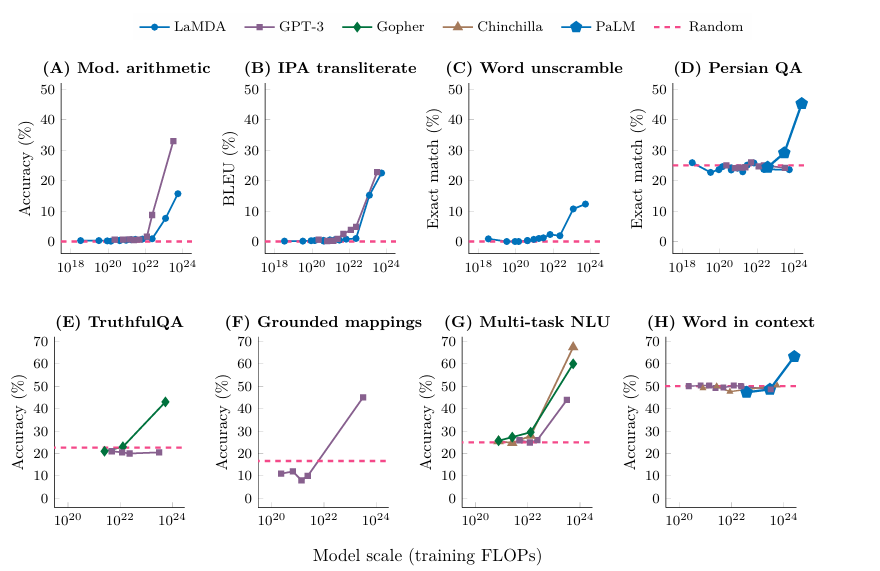
\includegraphics[width=0.8\textwidth]{../images/image.png} % Replace with your image path
    \caption{Model Scaling: Eight examples of emergence in the few-shot prompting setting. Each point is a separate model.The ability to perform a task via few-shot prompting is emergent when a language model achieves random performance until a certain scale,after which performance significantly increases to well-above random.Note that models that used more training compute also typically have more parameters—hence,we show ananalogous figure with number of model parameters instead of training FLOPs as the x-axis}
    \label{fig:model_scaling}
\end{figure}

\begin{figure}[htpb]
    \centering
    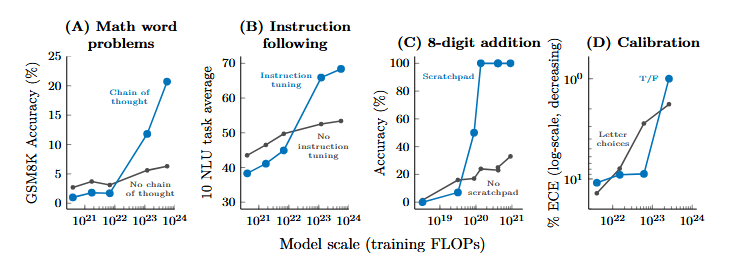
\includegraphics[width=0.5\textwidth]{../images/image-1.png} % Replace with your image path
    \caption{Augmented Prompting: Specialized prompting or finetuning methods can be emergent in that they do not have a positive
 effect until a certain model scale.}
    \label{fig:augmendted_prompting}
\end{figure}

\begin{figure}[htpb]
    \centering
    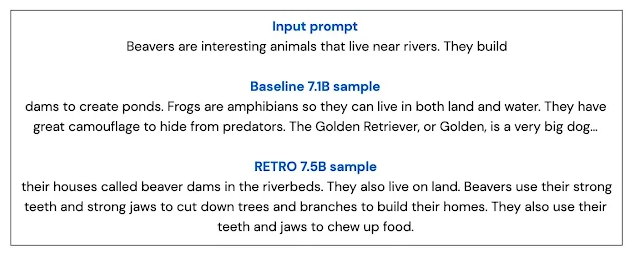
\includegraphics[width=0.6\textwidth]{../images/image-2.png} % Replace with your image path
    \caption{The RETRO model stays more on-topic than the baseline sample.Type image caption here (optional)}
    \label{fig:retro}
\end{figure}

The significance of this capability is further evidenced by the emergence of complex reasoning abilities in large-scale models. \parencite{wei_emergent_2022} discuss how phenomena like multi-step reasoning, often facilitated by techniques such as chain-of-thought prompting, become apparent in models typically exceeding 100 billion parameters as seen in Fig \ref{fig:model_scaling} and Fig \ref{fig:augmendted_prompting}. Such reasoning abilities frequently depend on understanding relationships across extended textual contexts, a feat well-supported by the Transformer architecture. Innovations like RETRO (Retrieval-Enhanced Transformer), introduced by \parencite{borgeaud_improving_2021}, augment Transformers with external retrieval mechanisms to enhance factuality and topical coherence. While retrieval provides supplementary information, the core Transformer architecture remains responsible for processing both the input and the retrieved passages, adeptly integrating their long-range contextual relationships as seen from Fig \ref{fig:retro}. Similarly, \parencite{khandelwal_generalization_2020} demonstrated that augmenting a pre-trained Transformer language model with a k-nearest neighbors model can improve predictions, particularly for rare patterns and factual knowledge, which often hinge on specific long-range contextual cues.

In summary, the continuous development and refinement of Transformer-based models, encompassing innovations like Switch Transformers for enhanced sparsity and retrieval-augmented models such as RETRO, underscore the fundamental strengths of this architecture. Its dual capabilities—efficient training on vast datasets and the inherent capacity to model complex, long-range relationships within text—have solidified the Transformer as the predominant backbone of modern large-scale language modeling. Ongoing research into areas such as instruction tuning \parencite{tay_long_2021,chung_scaling_2022}, model calibration, and more nuanced understanding of scaling behaviors, as seen in the work by \parencite{wei_emergent_2022} on emergent abilities, continues to build upon this powerful foundation, often seeking to more effectively train or adapt existing Transformer-based systems.


% Bibliography
\sloppy
\printbibliography

\end{document}